% --------------------------------------------------
% fichier includes/006-intro.tex
% première partie du travail : l'introduction
% premier titre numéroté
% numérotation en chiffre arabe
% --------------------------------------------------


\section{Introduction}

La mise en page du rapport de travail de Bachelor/Master comprend une marge de 2,5 cm en haut et en bas, ainsi qu’à droite. À gauche, une marge de 3,5 cm est requise pour permettre la reliure. La classe utilisée est \emph{article} et un espacement au-dessus des paragraphes de 9 pt. Le retrait au début du paragraphe est nul. Ces éléments sont renseignés dans le fichier \texttt{preamblule.tex} du répertoire \texttt{preambule/}.

Les titres suivants ne sont pas numérotés et sont centrés : déclaration, remerciements, résumé, liste des tableaux, liste des figures, bibliographie, annexes. Il faut utiliser l'astérisque (*) pour l'indiquer.

Tous les éléments entourés de crochets < > doivent être modifiés ou effacés et tous les crochets doivent être supprimés. Le premier fichier à modifier est \texttt{metadata.tex} dans le répertoire \texttt{preambule/}. Vous pouvez y indiquer le titre de votre travail, ainsi que votre prénom et votre nom. Dans le cas d'un travail à plusieurs, entrez les noms de tous les auteurs. Ces éléments sont repris à la page de la déclaration et dans les pieds de page. Par contre, il est nécessaire d'entrer votre prénom et votre nom dans le fichier \texttt{001-titre.tex} du répertoire \texttt{includes}.

Pour les listes à puces, utilisez l'environnement \texttt{itemize} :

\begin{itemize}[itemsep=0pt]
	\item Énumération
	\item Énumération
	\begin{itemize}[itemsep=0pt]
		\item Énumération
		\item Énumération
	\end{itemize}
	\item Énumération
\end{itemize}

Pour les listes numérotées, utiliser de manière similaire l'environnement \texttt{enumerate}.

Lorsque vous commencer une nouvelle section de niveau 1, faites-le sur une nouvelle page, grâce à la commande \verb?\newpage?. Cette commande est nécessaire, car dans ce modèle seules les sections sont utilisées, et non pas les parties et les chapitres.

Faites attention à la cohérence dans la numérotation des pages. Avant l'introduction, les pages sont numérotées en chiffres romains. À partir de l'introduction, la numérotation reprend à 1 en chiffres arabes et doit être continue sur tout le document, y compris dans les annexes.

Pour les figures, insérez-les sur le modèle ci-dessous. La commande \verb?\caption{}? sert à insérer la légende. Intégrez-la source dans la légende.

\begin{figure}[H]
	\noindent \begin{centering}
		\caption{Titre de la figure}
		\bigskip{}
			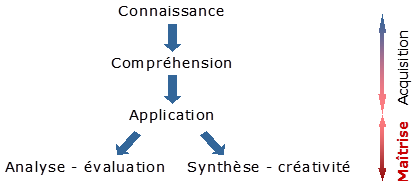
\includegraphics{images/image3.png}\bigskip{}
	\par \end{centering}
	\noindent \begin{raggedleft}
		(\cite[22]{bertholet_livres_1890}) % citation avec BibLaTeX 
	\par \end{raggedleft}
\end{figure}

Procédez de manière similiare avec un tableau :

\begin{table}[H]
	\noindent \begin{centering}
	\caption{Titre du tableau}
	\bigskip{}
		\begin{tabular}{|m{0.2\textwidth}|m{0.2\textwidth}|m{0.4\textwidth}|}
			\hline
			\textbf{Année} & \textbf{Ventes} & \textbf{Commandes} \\
			\hline
			2010 &  &  \\
			\hline
			2011 &  &  \\
			\hline
			2012 & & \\
			\hline
		\end{tabular}
		\bigskip{}
	\par\end{centering}
	\noindent \begin{raggedleft}
		(\cite[22]{bertholet_livres_1890}) % citation avec BibLaTeX
	\par\end{raggedleft}
\end{table}

Les notes en bas de page\footnote{Note de bas de page} servent à commenter un point. La fonction des notes de bas de page n'est pas de donner une référence bibliographique.

Les citations courtes sont insérée à l'intérieur d'un paragraphe, encadrée par des \enquote{guillemets}, qui sont ici générés par la commande \verb?\enquote{}?. La citation, comme la paraphrase, doit être suivie d'une parenthèse comprenant l'auteur et la date de la publication, ainsi que le numéro de la page d'où est tirée la partie citée ou paraphrasée : \enquote{Ceci est une citation courte, à l'intérieur d'un paragraphe.} (\cite[54]{bertholet_livres_1890}). Lorsque la citation est longue, elle fait l'objet d'un paragraphe qui lui est propre, avec une mise en forme adaptée.

La citation ci-dessus est réalisée avec la commande \verb?\begin{quote}?.

\begin{quote}
	Une citation peut se faire de deux manières : dans le corps du propos, elle est alors normalement entourée de guillemets, ou bien dans un paragraphe spécifique. Elle est alors	généralement présentée avec des marqueurs typographiques particuliers : changement de la taille de police, de la marge etc. (\cite[45]{rouquette_xelatex_2012})\end{quote}


